\documentclass[answers,addpoints]{exam}
\usepackage[margin=10mm]{geometry}
\usepackage{amsthm}
\usepackage{float} %  figure inside minipage 
\usepackage{ifthen,empheq}
\usepackage[]{graphicx}
\usepackage[]{minted}
\usepackage{amssymb}
\usepackage[multidot]{grffile}
\usepackage{pgfplots}
\usepackage{pgfplotstable}
\setlength{\headheight}{20pt}

\usepackage{tikz}
\usepgfplotslibrary{external}
\tikzexternalize[prefix=_tikz/,shell escape=-shell-escape]
\tikzset{external/system call={pdflatex \tikzexternalcheckshellescape -halt-on-error -interaction=batchmode -jobname "\image" "\texsource"}}
\immediate\write18{mkdir -p _tikz}

\title{Solution to HW3}
\author{Dilawar Singh}
\usepackage{hyperref}

\begin{document}
\Large
\maketitle

\begin{questions}

    \question[4]
    Refer to homework statement.

    \begin{parts}

        \part[2]

        \begin{solution}
            For every $y$, we can find at least one $x$ smaller than $y$ such that
            $f(x)$ is smaller than $f(y)$.

            \paragraph{negation} For any $y$, there is no $x$ smaller than $y$ such that
            $f(x)$ is smaller than $f(y)$.

            $\forall x$, $\nexists y$ such that if $x < y$ then $f(x) < f(y)$.

            Now, rewriting the previous statement, 

            For every $x$, there does not exists any $y$ such that $\ldots$.

            Using natural language, there could be multiple ways to write same thing
            . It is not easy to verify if all of those statements are equivalent.
            Mathematical symbols give a less error-prone way to operate on logical
            statements.
        \end{solution}

        \part[2]

        \begin{solution}

            There is at least one place where $f$ is 0. Or,
            There is at least one $x$ such that $f(x)=0$.

            \paragraph{Negation} There is no place where $f$ is zero. Or,
            $\forall x\; f(x) \neq 0$.

        \end{solution}

    \end{parts}


    \question[4]
    See the statement on google group.

    \begin{parts}

        \part[2] 
        \begin{solution}
            \paragraph{negation} $f$ is NOT increasing. $x < y \implies f(x) \ge f(y)$

        \end{solution}
        \part[2]
        \begin{solution}
            \paragraph{Negation} $f$ DOES NOT have a local maxima at $a$ i.e. in
            the $\delta$ neighbourhood of $a$, $f$ does not have this shape
            \tikz \draw[smooth ] (0,0.3) .. controls  (0.1,0) .. (0.2, 0.3); 

            $\forall \delta > 0$, $ \exists h \in \left(a-\delta, a+\delta
            \right)$, such that $f(a) \ge f(a+h)$.


        \end{solution}

    \end{parts}

    \question[12]

    The quadratic approximation goes like the following.

    $ f(x+h) = f(x) + h f'(x) + \frac{h^2}{2} f''(x) $. 

    And the solutions are plotted below. Note that this is not the replacement
    for algebraic analysis. 

    \begin{figure}[ht!]
    \begin{center}
        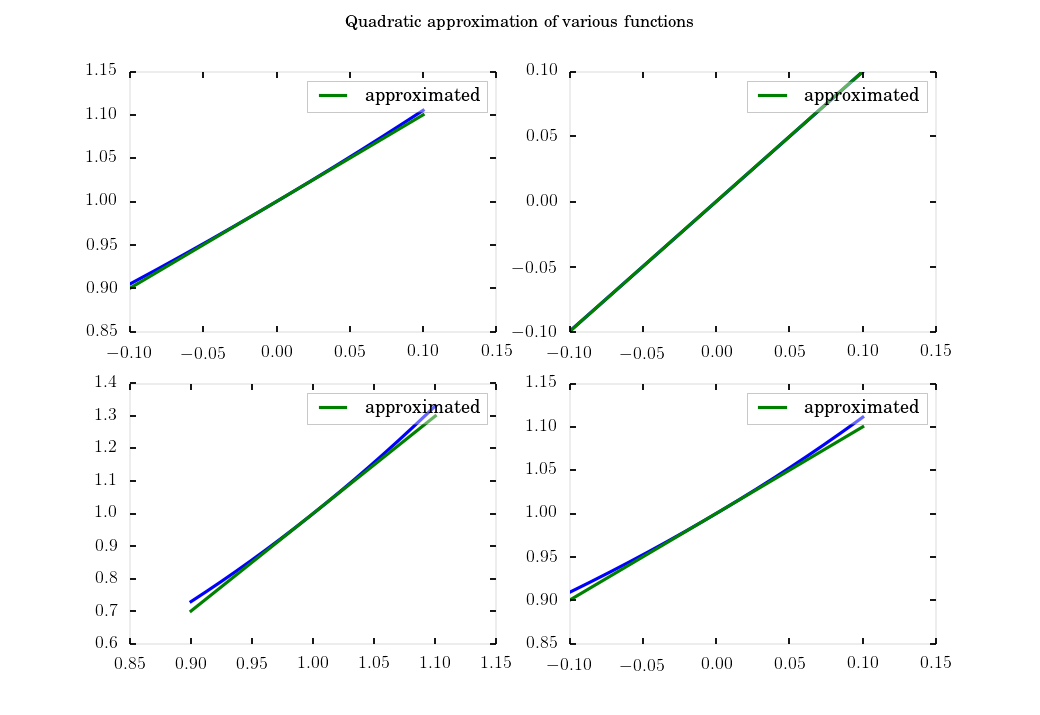
\includegraphics[width=1\textwidth]{./sol3.py.png}
    \end{center}
    \caption{ $f$ is $e^x$, $sin x$, $x^3$, and $\frac{1}{1-x}$ }
    \label{fig:}
    \end{figure}

    \question[12]

    \begin{parts}

        \part[4]
        \begin{solution}
            For $f$ to be even, we must have $f(x) = f(-x)$. Therefore, for all $x$
            such that $ax^3 + bx^2 + cx + d = -ax^3 + bx^3 -cx + d$, $f$ is even.
            That is $ax^3 + cx = 0 \implies x = 0, \pm \sqrt \frac{-c}{a} $.
            Similarly, for $f$ to be odd, $-ax^3 + bx^2 -cx+d = -ax^3 -bx^2 -cx-d$.
            That is $bx^2 +d = 0 \implies x = \pm \sqrt \frac{-d}{b}$.
        \end{solution}

        \part[12]
        \begin{solution}

        \end{solution}

        \part[4] 
        \begin{solution}

            $f'(x) = \lim_{h \rightarrow 0} \frac{ f(x+h) - f(x) }{h} $
            \begin{align}
                f'(-x) &= \lim_{h \rightarrow 0} \frac{ f(-x+h)) - f(-x) }{h} \\
                       &= \lim_{h \rightarrow 0} \frac{ f(-(x-h)) - f(x) }{h} \\
                       &= \lim_{h \rightarrow 0} \frac{ f(x-h) - f(x) }{h} \\
                       &= \lim_{h \rightarrow 0} - \frac{ f(x) - f(x-h) }{h} \\
                       &= \lim_{h \rightarrow 0} \frac{ f(x) - f(x-h) }{-h} \\
                       &= f'(x)
            \end{align}
            Or, $f'(-x) = f'(-x) \frac{d(-x)}{dx} $ (using chain rule). This
            gives us $f'(-x) = -f'(-x)$ therefore $f'(-x)$ is a even function.

            Similarly (i.e. I am too lazy to do any work), one can show that
            $g'$ is odd.
            
        \end{solution}


        \question[20]

            
        
    \end{parts}


\end{questions}


\end{document}          
